\newpage
\chapter{Modules}
This chapter is about the information page for the energy hub. The purpose of this page and the thought about design and how it will work is described here.
\section{Design Ideas}
The purpose of the hub page was to see what type of module there is connected to which ports, and to see the production versus the consumption. It is also possible to see some status of the energy hub. We also want a simple page without to many things to distract the users. To fulfil this we made 3 regions in the page window, one with the graph, one for data and status, and a third one for the modules.
\section{The Design}

\begin{figure}[h!]
	\center
		\setlength\fboxsep{0pt}
		\setlength\fboxrule{1pt}
		\fbox{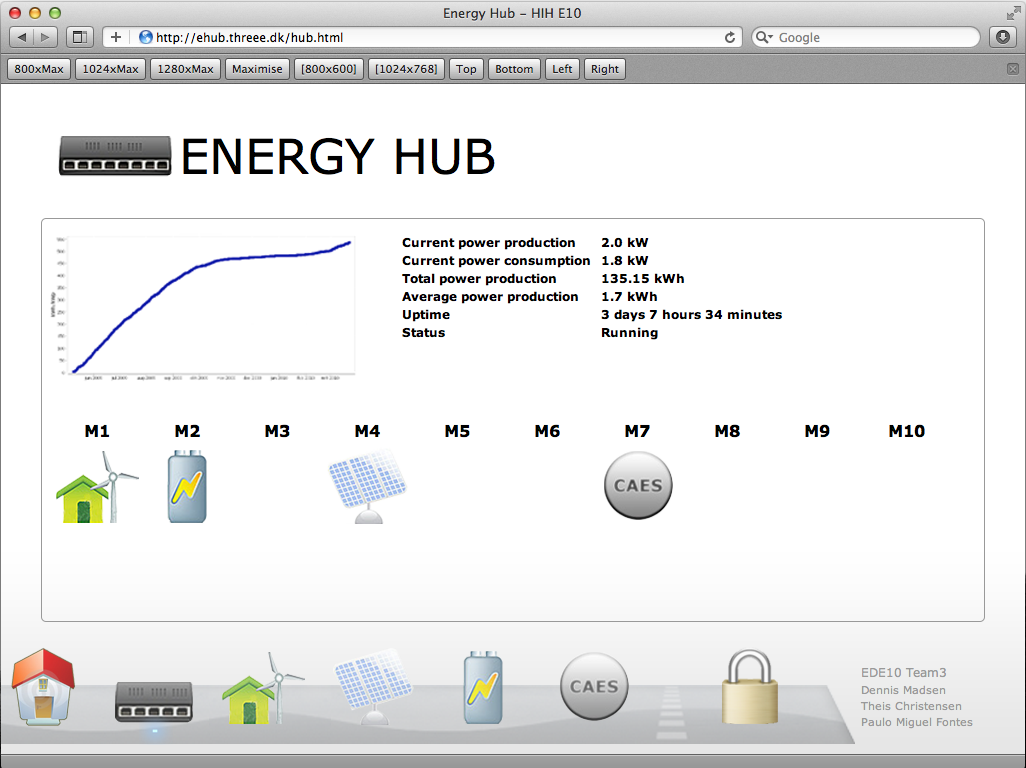
\includegraphics[width=0.6\textwidth]{images/screen_hub_page.png}}
   	\caption{Picture of the hub page.}
   	\label{fig:hub_page_design}
\end{figure}
This is how out design turns out. It fulfil the purpose and out own requirements for the design.
\section{Code layout}
Here is a description of the code settings and layout that we use to our webpage.
\subsection{Doctype}
In this project we are using the XHTML 1.0 Strict document type. The DOCTYPE declaration tells the browser how to interpret the code in which the site is written. It should be written at the first line in every valid html file, as seen in the code below. This type has every feature of the HTML. The markup must be written as well formed XML. Strict, in contrary to Transitional, document types does not include deprecated tags (e.g. \textless font\textgreater , \textless target\textgreater), so all our styling is made in the CSS style sheet.
\begin{lstlisting}
<!DOCTYPE html PUBLIC "-//W3C//DTD XHTML 1.0 Strict//EN" "http://www.w3.org/TR/xhtml1/DTD/xhtml1-strict.dtd">
\end{lstlisting}

\subsection{Meta tag}
The meta tags tell something about the data on the page. In the first line we set the content type to "text/html" that means that the browser will show the page as normal, we also set the charset in that line to "UTF-8". In the second line we determine the width of the viewport this makes the page expand with the browser, we also set that the user can not scale the page.
\begin{lstlisting}
<meta http-equiv="Content-Type" content="text/html; charset=UTF-8" />
<meta name="viewport" content="width=device-width, initital-scale=1, user-scalable=no" />
\end{lstlisting}

\section{Code explanation}
Here the code will be described and shown in pieces
\subsection{Division}
html code
\begin{lstlisting}
<div class="modules" id="M1">		
	M1<br />
	<a href="wind.html"> <img src="pic/dock_wind.png"		alt="WIND_module"/> 	</a>
</div>
<div class="modules" id="M2">
	M2<br />
	<a href="battery.html"> <img src="pic/dock_bat.png" 	alt="battery_module"/>	</a>
</div>
\end{lstlisting}
css code
\begin{lstlisting}[language=CSS]
/*MODULES*/
.modules {/*Classe settings*/
	text-align: center;
	font-weight: bold;
	position:inherit;
	height: 120px;
	width: 90px;
	top: 200px;
}
/*Setting for single id*/
#M1	{left: 10px;}
#M2	{left: 100px;}
\end{lstlisting}

\subsection{headings}
When we want to make headlines in html we can use headings tags (\textless h1\textgreater  to\textless h6\textgreater). We can then define how we want the specific headings tags to look like in the css file. We are using the h1 tag in the html code below.
\begin{lstlisting}
<div id="header">
	<img src="pic/hub.png" alt="HUB_module"/>
	<h1>ENERGY HUB</h1>
</div>
\end{lstlisting}
The code below is the css code to design the h1 tag from the html code above. In the css code we set the font size of h1 in the header division, we also set the top padding which set the space from the element above the heading.
\begin{lstlisting}[language=CSS]
#header h1{ font-size: 48px; padding-top: 35px;}
\end{lstlisting}

\subsection{Table}
html code
\begin{lstlisting}
<div id="status"><!-- Table for the hub status-->
	<table>
		<tr>
			<td>Current power production</td><td>2.0 kW</td>
		</tr>
		<tr>
			<td>Current power consumption</td><td>1.8 kW</td>
		</tr>
		<tr>
			<td>Total power production</td><td>135.15 kWh</td>
		</tr>
		<tr>
			<td>Average power production</td><td>1.7 kWh</td>
		</tr>
		<tr>
			<td>Uptime</td><td>3 days 7 hours 34 minutes</td>
		</tr>
		<tr>
			<td>Status</td><td>Running</td>
		</tr>
	</table>
</div>
\end{lstlisting}
css code
\begin{lstlisting}[language=CSS]
#status td {
	padding-left: 10px;
	font-weight: bold;
	font-size: 12px;
}
\end{lstlisting}

\subsection{General tags}
html code
\begin{lstlisting}

\end{lstlisting}
css code
\begin{lstlisting}[language=CSS]

\end{lstlisting}